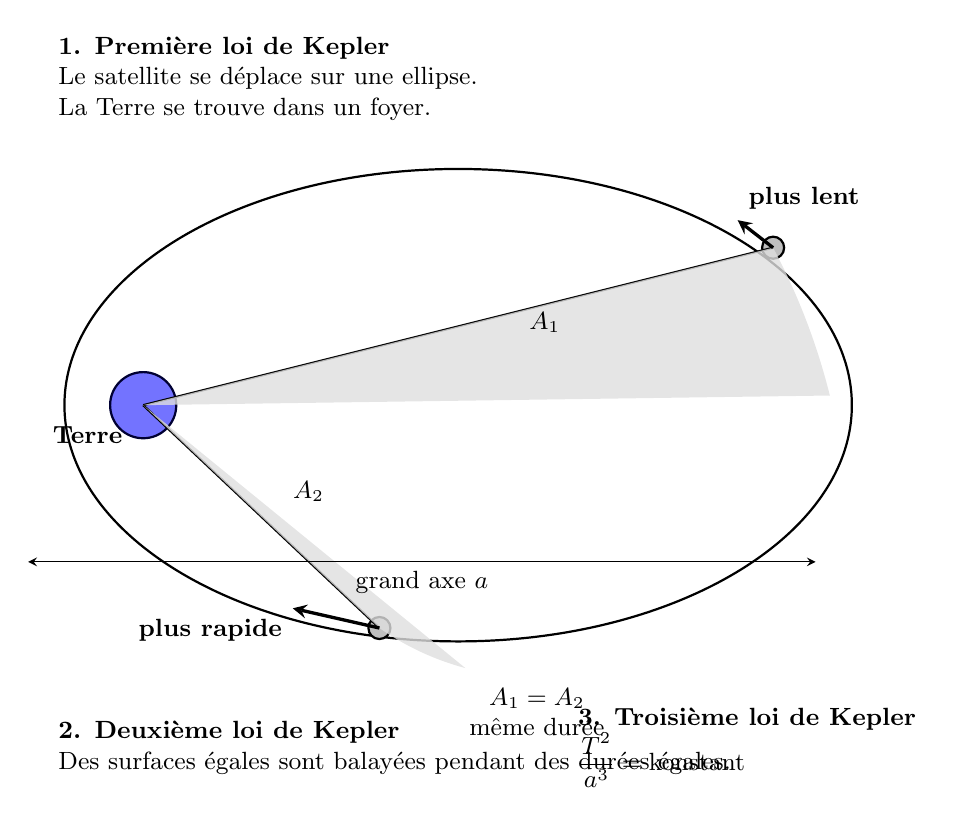
\begin{tikzpicture}[
    scale=1.0,
    >=stealth,
    every node/.style={font=\small}
]

% ============================================================
% Elliptische Satellitenbahn
% ============================================================

% Halbachsen
\def\a{5}
\def\b{3}
\def\c{4}

% Terre im Brennpunkt
\coordinate (Earth) at (-\c,0);

% Ellipse
\draw[thick] (0,0) ellipse (\a cm and \b cm);

% ============================================================
% Terre
% ============================================================

\filldraw[
    fill=blue!55,
    draw=blue!20!black,
    thick
]
(Earth) circle (0.42cm);

\node[below left=4pt] at (Earth)
    {\textbf{Terre}};

% ============================================================
% Zwei Satellitenpositionen
% ============================================================

% Position 1: weit von der Terre entfernt
\coordinate (S1) at (4.0,2.0);

% Position 2: näher bei der Terre
\coordinate (S2) at (-1.0,-2.83);

% Satellit an Position 1
\filldraw[
    fill=gray!50,
    draw=black,
    thick
]
(S1) circle (0.14cm);

% Satellit an Position 2
\filldraw[
    fill=gray!50,
    draw=black,
    thick
]
(S2) circle (0.14cm);

% ============================================================
% Fahrstrahlen
% ============================================================

\draw[thick] (Earth) -- (S1);
\draw[thick] (Earth) -- (S2);

% ============================================================
% Überstrichene Flächen
%
% Die Flächen werden schematisch als gleich grosse
% Sektoren dargestellt.
% ============================================================

% Fläche A1
\fill[
    gray!25,
    opacity=0.8
]
(Earth) --
(4.0,2.0)
arc[
    start angle=28,
    end angle=14,
    x radius=8.25cm,
    y radius=8.25cm
] -- cycle;

% Fläche A2
\fill[
    gray!25,
    opacity=0.8
]
(Earth) --
(-1.0,-2.83)
arc[
    start angle=-125,
    end angle=-105,
    x radius=3.47cm,
    y radius=3.47cm
] -- cycle;

% ============================================================
% Geschwindigkeiten
% ============================================================

% Geschwindigkeitsvektor nahe Terre
\draw[very thick,->]
    (S2) -- ++(-1.1,0.25)
    node[below left] {\textbf{plus rapide}};

% Geschwindigkeitsvektor weit entfernt
\draw[very thick,->]
    (S1) -- ++(-0.45,0.35)
    node[above right] {\textbf{plus lent}};

% ============================================================
% Beschriftung der beiden Flächen
% ============================================================

\node at (1.1,1.05)
    {$A_1$};

\node at (-1.9,-1.1)
    {$A_2$};

\node[align=center] at (1.0,-3.9)
    {$A_1=A_2$\\
     même durée};

% ============================================================
% Grosse Halbachse
% ============================================================

\draw[<->,thin]
    (-5.46,-1.99) -- (4.54,-1.99)
    node[midway,below] {grand axe $a$};

% ============================================================
% Keplersche Gesetze
% ============================================================

\node[
    align=left,
    anchor=west
] at (-5.2,4.15)
{
\textbf{1. Première loi de Kepler}\\
Le satellite se déplace sur une ellipse.\\
La Terre se trouve dans un foyer.
};

\node[
    align=left,
    anchor=west
] at (-5.2,-4.35)
{
\textbf{2. Deuxième loi de Kepler}\\
Des surfaces égales sont balayées pendant des durées égales.
};

\node[
    align=left,
    anchor=west
] at (1.4,-4.35)
{
\textbf{3. Troisième loi de Kepler}\\
$\displaystyle \frac{T^2}{a^3}=\mathrm{konstant}$
};

\end{tikzpicture}